\documentclass[10pt,a4j]{article}
%\usepackage{graphicx,wrapfig}
\usepackage{graphicx}
\setlength{\topmargin}{-1.5cm}
\setlength{\textwidth}{16.5cm}
\setlength{\textheight}{25.2cm}
\newlength{\minitwocolumn}
\setlength{\minitwocolumn}{0.5\textwidth}
\addtolength{\minitwocolumn}{-\columnsep}
%\addtolength{\baselineskip}{-0.1\baselineskip}
%
\def\Mmaru#1{{\ooalign{\hfil#1\/\hfil\crcr
\raise.167ex\hbox{\mathhexbox 20D}}}}
%
\begin{document}
\newcommand{\fat}[1]{\mbox{\boldmath $#1$}}
\newcommand{\D}{\partial}
\newcommand{\w}{\omega}
\newcommand{\ga}{\alpha}
\newcommand{\gb}{\beta}
\newcommand{\gx}{\xi}
\newcommand{\gz}{\zeta}
\newcommand{\vhat}[1]{\hat{\fat{#1}}}
\newcommand{\spc}{\vspace{0.7\baselineskip}}
\newcommand{\halfspc}{\vspace{0.3\baselineskip}}
\bibliographystyle{unsrt}
%\pagestyle{empty}
\newcommand{\twofig}[2]
 {
   \begin{figure}
     \begin{minipage}[t]{\minitwocolumn}
         \begin{center}   #1
         \end{center}
     \end{minipage}
         \hspace{\columnsep}
     \begin{minipage}[t]{\minitwocolumn}
         \begin{center} #2
         \end{center}
     \end{minipage}
   \end{figure}
 }
%%%%%%%%%%%%%%%%%%%%%%%%%%%%%%%%%
%\vspace*{\baselineskip}
\begin{center}
	{\Large \bf Lecture Note 1 for Civil Engineering I \\ - an introduction to structural mechanics}  
\end{center}
%%%%%%%%%%%%%%%%%%%%%%%%%%%%%%%%%%%%%%%%%%%%%%%%%%%%%%%%%%%%%%%%
\section{Review of Vector Algebra}
\subsection{Scalar and vector quantites}
A scalar is a quantitiy that has only a magnitude, while a vector has 
both magnitude(or length) and direction.
%The magnitude can either be positive or negative. 
The examples of scalar quantities frequently used in physics and engineering 
are mass, temperature, concentration, length, weight and so on.
%Vector is a quantity that has both a magnitude and direction. 
The examples of vector quantities are displacement, velocity, acceleration, 
force, heat flux, mass flux, electric poloarization, etc. 
It is sometimes useful to denote vectors by arrows typically when 
the gemterical relationship among the vectors is of interest.
In that situation, the magnitude and direction of a vector 
are indicated by the length and the orientation of the arrow, 
respectively, as shown in Fig.\ref{fig:fig1_1}. 
For more rigorous discussion, however, symbolic representations 
of vectors are far more convenient. 
\begin{figure}[h]
	\begin{center}
	\includegraphics[width=0.2\linewidth]{arrow.eps} 
	\end{center}
	\caption{A vector $\fat{a}$ shown graphically by an arrow.} 
	\label{fig:fig1_1}
\end{figure}
To denote vector quantities in typed manuscripts symbolically, boldface letters such 
as $\fat{x},\fat{u},\fat{v},\dots$ are used instead of writting simply as $x, u$ and $v$.
It is important not to confuse vectors and scalars since they are qualitatively different entities.
To denote the magnitude of vector $\fat{a}$, we either write $|\fat{a}|$ or simply $a$.
Unlike scalars, vector length is always greater than or equal to zero(i.e. $|\fat{a}| \geq 0$).
If $\fat{a}$ has a unit magnitude ($|\fat{a}|=a=1$), then $\fat{a}$ is said to be a unit vector. 
If $|\fat{a}|=0$, it is said to be zero vector writting $\fat{a}=\fat{0}$. 
Note that the direction is not defined for zero vector.
\subsection{Vector Identity}
Two vectors $\fat{a}$ and $\fat{b}$ are considered identical 
if their magnitude and direction are equal.
In that case, we write $\fat{a}=\fat{b}$ regardless of their locations(see, Fig.\ref{fig:fig1_2}-(a)). 
For example, when two forces ($\fat{f}, \fat{g}$) of equal magnitude and direction 
are acting to two different locations on a body, 
$\fat{f}$ and $\fat{g}$ are considered mathematically identical although they 
are physically different forces(Fig.\ref{fig:fig1_2}-(b)).
The exception of this rule is position vectors. 
The origin of position vectors are always taken at 
the origin of a predefined coordinate as illustrated in Fig.\ref{fig:fig1_2}-(c).
The position vectors should be defined in that way since the correspondance between 
spatial points and position vectors must be one-to-one. 
\begin{figure}[h]
	\begin{center}
	\includegraphics[width=0.7\linewidth]{identity.eps} 
	\end{center}
	\caption{(a),(b)Pairs of mathematically identical vectors. 
	(c) An illustration of position vectors.} 
	\label{fig:fig1_2}
\end{figure}
\subsection{Basic Algebraic Operation on Vectors}
The most fundamental algebraic operations on vectors are (1) scalar mutiplication 
and (2) vector addition, which are introduced as follows.
\subsubsection{Scalar multiplication}
A multiplication between a scalar $s$ and a vector $a$ is called "scalar multiplication" 
and is written as $s\fat{a}$. For $s>0$, scalar multiplication $s\fat{a}$ strecthes (compresses) $\fat{a}$ 
by $s$ times if $s \geq 1 (s<1)$ without changing the direction(see Fig.\ref{fig:fig1_3}-(a) and (b)).
When $s<0$, the scalar multiplication first reverset the directoin and then stretches or compresses 
$\fat{a}$ by $|s|$ times(see Fig.\ref{fig:fig1_3}-(c) and (d)).
Some obvious consequences of this definition of scalar multiplication are:
\begin{itemize}
\item 
	$1\fat{a}=\fat{a}$,
\item 
	$0\fat{a}=\fat{0}$,
\item
	(st)\fat{a}=s(t\fat{a}),
\end{itemize}
where $s$ and $t$ are arbitrary scalars. 
\begin{figure}[h]
	\begin{center}
	\includegraphics[width=0.7\linewidth]{smul.eps} 
	\end{center}
	\caption{The results of scalar multiplications $s\fat{a}$ dependent on the scalar $s$.} 
	\label{fig:fig1_3}
\end{figure}
\subsubsection{Vector addition}
Vector addition is an operation that produces a new vector by connecting a pair of vectors. 
If we let $\fat{a}$ and $\fat{b}$ be two arbitrary vectors, 
we can form a directed broken line by connecting the tail of one vector with 
the head of the other. The sum $\fat{a}+\fat{b}$ is defined to be a vector 
extending from the origin of the broken line to its head.
Followings are direct consenqueces of this definition.
\begin{equation}
	\fat{a}+\fat{0} = \fat{0}+\fat{a}=\fat{a}. 
\end{equation}
\begin{equation}
	\left(s+t \right)\fat{a}= s\fat{a}+ t\fat{a}
	\label{eqn:}
\end{equation}
\begin{equation}
	s(\fat{a}+\fat{b})=s\fat{a}+s\fat{b}
	\label{eqn:}
\end{equation}
Note that vector addition is "commutative" since 
\begin{equation}
	\fat{a}+\fat{b}=\fat{b}+\fat{a}
\end{equation}
alwyas hold true. This means the order of summation can be exchanged. 
Clearly, we can add more than two vectors by repeating the pair wise vectors addition.
For example, we can perform summation of three vectors either by 
\[
	\fat{a}+\left( \fat{b}+\fat{c} \right)
\]
or by 
\[
	\left( \fat{a}+\fat{b} \right) + \fat{c}.
\]
We can prove graphically that the addition by result in a same vector. Hence, 
\begin{equation}
	\fat{a}+\left( \fat{b}+\fat{c} \right)
	=
	\left( \fat{a}+\fat{b} \right) + \fat{c}.
\end{equation}
\begin{figure}[h]
	\begin{center}
	\includegraphics[width=0.6\linewidth]{vadd.eps} 
	\end{center}
	\caption{(a) Vector addition $\fat{a}+\fat{b}$ and 
	(b) Vector subtraction $\fat{a}-\fat{b}$.} 
	\label{fig:1_4}
\end{figure}
\subsection{Inner (or Dot) product} 
Another useful vector multiplication is inner product or dot product.
The inner product of $\fat{a}$ and $\fat{b}$ is written as $\fat{a}\cdot\fat{b}$, 
and may be defined by 
\begin{equation}
	\fat{a}\cdot\fat{b}=|\fat{a}||\fat{b}|\cos\theta
\end{equation}
where $\theta$ is the angle between $\fat{a}$ and $\fat{b}$ (see Fig.\ref{fig:fig1_5}-(a)). 
Clearly, the inner product is commutative that the order of multiplication 
can be changed.
\begin{equation}
	\fat{a}\cdot\fat{b}
	=
	\fat{b}\cdot\fat{a}, 
	\label{eqn:}
\end{equation}
and linear in the following sense.
\begin{equation}
	\left(s\fat{a}+t\fat{b}\right)\cdot\fat{c}
	=
	s(\fat{a}\cdot\fat{c})+t(\fat{b}\cdot \fat{c})
	\label{eqn:}
\end{equation}
Numerically, the inner product can either be positive or negative 
depending on the angle $\theta$.
\begin{equation}
	\fat{a}\cdot\fat{b}
	=
	\left\{
	\begin{array}{cc}
		>0 & ( |\theta|< \pi/2) \\
		<0 & ( |\theta| > \pi/2)
	\end{array}
	\right.
	.
	\label{eqn:}
\end{equation}
When $\fat{a}\cdot\fat{b}=0$, that is when $\theta=\pi/2$, $\fat{a}$ and $\fat{b}$ 
are said to be mutual orthogonal.
Inner prodocut of unit vectors are often of particluar interest. 
If $\fat{a}$ is a unit vector, $\fat{a}\cdot\fat{b}$ gives a projection of $\fat{b}$ 
to the line colinear to $\fat{a}$ as shown in Fig.\ref{fig:fig1_5}. 
\begin{figure}[h]
	\begin{center}
	\includegraphics[width=0.4\linewidth]{iprod.eps} 
	\end{center}
	\caption{The angle $\theta$ formed by vectors $\fat{a}$ and $\fat{b}$. 
	(b) A projection of $\fat{b}$ to the line colinear to a unit vector $\fat{a}$.} 
	\label{fig:fig1_5}
\end{figure}
%%%%%%%%%%%%5
\subsection{Cross product} 
For vectors in s three dimensional space, yet another vector multiplication called 
cross (or exterior) product may be introduced. For given pair of vectors $\fat{a}$ and $\fat{b}$, 
the cross product denoted by $\times$ produces a third vector $\fat{a}\times \fat{b}$. 
The defining propertis of the cross product are as follows. 
\begin{equation}
	\fat{a}\times \fat{b}= -\left(\fat{b} \times \fat{a} \right)
	\label{eqn:asym}
\end{equation}
\begin{equation}
	\left(\fat{a}+\fat{b}\right)\times \fat{c}
	=
	\fat{a}\times \fat{c}+ \fat{b}\times \fat{c}
	\label{eqn:}
\end{equation}
\begin{equation}
	\left(\fat{a}\times\fat{b}\right)\cdot\fat{a} =
	\left(\fat{a}\times\fat{b}\right)\cdot\fat{b} =0 
	\label{eqn:ortho}
\end{equation}
\begin{equation}
	\left|\fat{a}\times \fat{b} \right|^2=|\fat{a}|^2|\fat{b}|^2-\left(\fat{a}\cdot\fat{b}\right)^2
	\label{eqn:area}
\end{equation}
In addition to the properties (\ref{eqn:asym})-(\ref{eqn:area}), it is usually 
required that the tuple:
\begin{equation}
	\left(\fat{a},\fat{b},\fat{a}\times \fat{b} \right)
	\label{eqn:vtuple}
\end{equation}
forms a right-handed system.
Note that property (\ref{eqn:asym}) implies 
\begin{equation}
	\fat{a}\times \fat{a}=\fat{0}
	\label{eqn:}
\end{equation}
The motivation behind the above properties is evident. 
As illustrated in Fig.\ref{fig:fig1_6}, the cross product are orthogonal to 
both $\fat{a}$ and $\fat{b}$. Thus $\fat{a}\times \fat{b}$ is perpendicular 
to the pararellogram formed by $\fat{a}$ and $\fat{b}$. 
The direction of $\fat{a}\times\fat{b}$ is chosen so that the tuple (\ref{eqn:vtuple}) 
forms a right-handed system, while the length is taken to be the area of 
the parallelogram. 
\begin{figure}[h]
	\begin{center}
	\includegraphics[width=0.4\linewidth]{eprod.eps} 
	\end{center}
	\caption{Gemetrical configuration of a vector cross product 
	$\fat{a}\times\fat{b}$ relative to $\fat{a}$ and $\fat{b}$.} 
	\label{fig:fig1_6}
\end{figure}
\subsection{Vector components}
When performing a vector algebra, we almost always decompose the vectors into components. 
For the decompositoin it is convenient to introduce a coordinate. 
Among variety of different coordinate systems, Cartesian coordinates are 
by far the most fundamental and most convenient.
If we place our vector in a Catesian coordinate space so that the origin of the 
vector comes to the orgin of the coordinate, we can determin the coordinates 
that the vector is pointing at. 
In Fig.\ref{fig:fig1_7}, Cartesian coordinates in 2 and 3 dimensional space 
are illustrated.
Since the correspondance between the coordinates and vector is one-to-one, we can 
identify the vector $\fat{a}$ with the coordinates $(a_x,a_y)$. Thus we write a 
vector in 2 dimensional space as
\[
	\fat{a}=(a_x, a_y).
\]
Note that $a_x$ and $a_y$ are the projected length of $\fat{a}$ to each coordinate axis.
If we write the projection of $\fat{a}$ to $x$ and $y$ axes as $\fat{a}_x$ and $\fat{a}_y$ respectively, 
then it is clear that 
\begin{equation}
	|\fat{a}_x|=a_x, \ \ |\fat{a}_y|=a_y.
	\label{eqn:}
\end{equation}
Moreover, it can also be verified that 
\begin{equation}
	\fat{a}=\fat{a}_x+\fat{a}_y
	\label{eqn:}
\end{equation}
holds.  This means $\fat{a}$ can be decomposed into componets. 
In this sence, the coordinates $(a_x,a_y)$ are also called vector components. 
More specifically, $a_x$ and $a_y$ are called $x$ and $y$ components, respectively.
Clearly, the third coordnate is required for the description of vectors in 3D space. 
However, the above discussion applies equally to vectors in 3D except the need for 
 the extra coordinate and vector component.
\begin{figure}[h]
	\begin{center}
	\includegraphics[width=0.5\linewidth]{components.eps} 
	\end{center}
	\caption{Cartesian coordinates and vector components.} 
	\label{fig:fig1_7}
\end{figure}
\subsection{Component-wise operations}
Let
\begin{equation}
	\fat{a}=\left(a_x,a_y \right), \ \ 
	\fat{b}=\left(b_x,b_y \right)
	\label{eqn:}
\end{equation}
and let $s$ be an arbitrary scalar.
\begin{equation}
	s\fat{a}
	=
	\left\{
		\begin{array}{c}
			sa_x \\
			sa_y 
		\end{array}
	\right\}
	\label{eqn:}
\end{equation}
\begin{equation}
	\fat{a}
	+
	\fat{b}
	=
	\left\{
		\begin{array}{c}
			a_x \\
			a_y 
		\end{array}
	\right\}
	+
	\left\{
		\begin{array}{c}
			b_x \\
			b_y 
		\end{array}
	\right\}
	=
	\left\{
		\begin{array}{c}
			a_x+b_x \\
			a_y+b_y
		\end{array}
	\right\}
	\label{eqn:}
\end{equation}
\begin{equation}
	\fat{a} \cdot \fat{b}
	=
	\left\{
		\begin{array}{c}
			a_x \\
			a_y 
		\end{array}
	\right\}
	\cdot
	\left\{
		\begin{array}{c}
			b_x \\
			b_y 
		\end{array}
	\right\}
	= a_xb_x+a_yb_y
	\label{eqn:}
\end{equation}
\begin{equation}
	\left| \fat{a} \right|^2 = a_x^2 + a_y^2
	\label{eqn:}
\end{equation}
\begin{equation}
	\left| \fat{a}-\fat{b} \right|^2
	=
	\left| \fat{a} \right|^2
	\left| \fat{b} \right|^2
	+2
	\left| \fat{a} \right| \left| \fat{b} \right| \cos\theta
	\label{eqn:}
\end{equation}
\begin{equation}
	(a_x-b_x)^2+(a_y-b_y)^2
	=
	(a_x^2+a_y^2)+(b_x^2+b_y^2) -2\fat{a}\cdot\fat{b}
	\label{eqn:}
\end{equation}
%%%%%%%%%%%%%%%%%%%%%%%%%%%%%%%%%%%%%%%%%%%%%%
\section{Newton's law of motion}
Newton discovered the laws that govern the motion of planetary bodies. 
The governing laws he found are 
\begin{enumerate}
	\item Existence of an intertia system
	\item Conservation of linear momentum
	\item The law of action and reaction,
\end{enumerate}
which are collectively called as the Newton's laws of motion. 
In his effort of understanding the planetary motion, he modeled the planetary 
bodis by mass poits neglecting the size of the bodies. 
Although considerable extentions have been made since his days to deal with a 
 deformable bodies of finite size, the Newton's laws themselves have not been modified. 
Structural mechanics is built entirely on the basis of Newton's mechanics. 
The followings are reasonably accurate statements of the three Newton's law for our present application. 
\begin{enumerate}
\item 
	There exsist a coordinate system in which we can observe bodies move at a constant velocity 
	if no force is being exserted the bodies. Such coordinate system is called an "inertia system".
\item
	The time rate of change in the linear momentum of a body is equal to the force applied to it.
\item
	If two bodies are excersizing forces each other, the forces applied from one body to 
	the other is equal in magnitude but opposite in direction.
\end{enumerate}
Among the three laws, the 2nd law is of our primary interest, and then comes the third. 
To state the 2nd law more rigorously, let $m$ be the mass, and let $\fat{v}$ and $\fat{f}$ 
be the velocity and the force, respectively. Then the linear momentum is given by $m\fat{v}$, 
and the 2nd law can be written as 
\begin{equation}
	\fat{f}=\frac{d}{dt}\left(m\fat{v}\right)
	\label{eqn:2nd_law}
\end{equation}
where $t$ is time.
The 3rd law is concerend with two interacting body, say body A and B. 
If body A is applying a force $\fat{f}_{AB}$ to body B, 
then the 3rd law tells us that body A is under the force $\fat{f}_{BA}$ 
of same magnitude acting in the opposite direction. Thus, 
the precise statement is written as 
\begin{equation}
	\fat{f}_{AB}=-\fat{f}_{BA}.
	\label{eqn:}
\end{equation}
Note that either or both body A and B could be a floor or a wall of infinite mass. 
%%%%%%%%%%%%%%%%%%%%
\section{Equation of Motion}
In Newton's mechanics, mass $m$ is a clearly defined constant. 
Therefore, eq.(\ref{eqn:2nd_law}) can be written equivalently as 
\begin{equation}
	\fat{f}=m \frac{d\fat{v}}{dt}=m\fat{\alpha}, \ \ \left(\alpha=\frac{d\fat{v}}{dt}\right)
	\label{eqn:eq_mot}
\end{equation}
where $\fat{\alpha}$ is the acceleration.
Equation (\ref{eq_mot}) is more commonly called as "equation of motion".
When $\fat{f}=\fat{0}$, eq.(\ref{fig:2nd_law}) is reduced to 
\begin{equation}
	\frac{d}{dt}\left(m\fat{v}\right)=\fat{0} \ \ \Rightarrow \ \ 
	m\fat{v}=const.
	\label{eqn:mv_cnst}
\end{equation}
In this case, the linear momentum does not chage over time. This is the reason why 
the 2nd law is often reffered to as a conservation law of linear momentum.
On the other hand, if the velocity is known not chaging over time, then the force 
should vanish reducing the equation of motion to  
\begin{equation}
	\fat{f}=\fat{0}.
	\label{eqn:equiv0}
\end{equation}
It seems that eq.(\ref{eqn:equiv0}) is a trivial relation. 
When multiple forces are acting to the body, however, $\fat{f}$ 
must be considered as the sum of all forces. To address this issue, 
let the forces applied to the body be $\fat{f}_1, \fat{f}_2,\dots \fat{f}_n$, then 
eq.(\ref{eqn:equiv0}) can be written more appropriately as 
\begin{equation}
	\sum_{i=1}^n\fat{f}_i=\fat{0}.
	\label{eqn:equiv}
\end{equation}
Equation (\ref{eqn:equiv}) is called an "equilibrium equation" or "equilibrium condition". 
\section{Dynamics and statics}
A branch of mechanics that studies time varying motion and deformation of materials is 
called "dynamics". Dynamics is one of the most important conner stones of such scientific 
 disciplines as vibration, acoustics, and seismology.
The other branch of mechanics is called "statics", which studies the action of forces 
to materials in a static equilibirum. When narrowly defined, structural mechanics is fallen 
in the caterogy of statics. A structural mechanics dedicated to the analysis of structural vibration 
is called structural dynamics. 
In this class, we're going to learn basic techniques to study strcutures in static equilibrium 
under a given set of external forces. 
This class is therefore concerned with a "static" structural mechanics, and derive everything 
from the equilibrium equation (\ref{eqn:equiv}). 
\section{Problems}
\section*{Solved Problems}
\begin{itemize}
\item
Exercise 1-1:\\
Verify that the vector addition is associative,i.e., 
\[
	\fat{a}+(\fat{b}+\fat{c})=
		(\fat{a}+\fat{b})+\fat{c}
\]
using graphic representation of vectors. 
\item
Exercise 1-2:\\
For vectors $\fat{a}$ and $\fat{b}$ given in Fig.\ref{fig:fig1_1}, 
work out $\fat{a}+\fat{b}$ by the component based 
		method when  $|\fat{a}|=1$ and $|\fat{b}|=2$.
		Also, obtain $|\fat{a}+\fat{b}|$ numerically.
\item
Exercise 1-3:\\
		For vectors given in Fig.\ref{fig:fig1_2} Prove that 
	\[
		\fat{a}+\fat{b}+\fat{c}=\fat{0}
	\]
		if $|\fat{a}|=|\fat{b}|=|\fat{c}|$.
\item
Exercise 1-4:\\
Suppose that a perfectly rigid bar AB is supported horizontally by a wall
 as shown in Fig.\ref{fig:fig1_3}, and is subjected to infinitely many 
vertical forces $\fat{f}_i (i=1,2,...)$ whose magnitude decreases monotonically as 
\[
 \frac{
	|\fat{f}_{i+1}|
	}{
	|\fat{f}_i|
}
	=\frac{9}{10} 
\]
Determine the direction and the magnitude of the total force acting on the bar. 
\item
Exercise 1-5:\\
	Suppose that an iron weight is hung from a ceiling by a string AB as shown in Fig.\ref{fig:fig1_4}-(a). 
	Determine the magnitude of the horizontal force $F$ required to hold the weight as 
	in the position shown in Fig\ref{fig:fig1_4}-(b).
	Note that $m$ is mass and $g$ is gravity constant.  
\end{itemize}
\begin{figure}[h]
	\begin{center}
	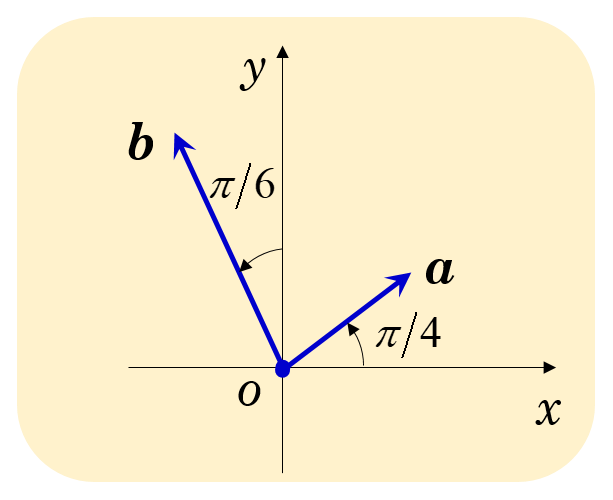
\includegraphics[width=0.3\linewidth]{fig1_1.eps} 
	\end{center}
	\caption{Vectors $\fat{a}$ and $\fat{b}$ in 2-dimensional space with an
	xy Cartesian coordinate system.}
	\label{fig:fig1_1}
\end{figure}
\begin{figure}[h]
	\begin{center}
	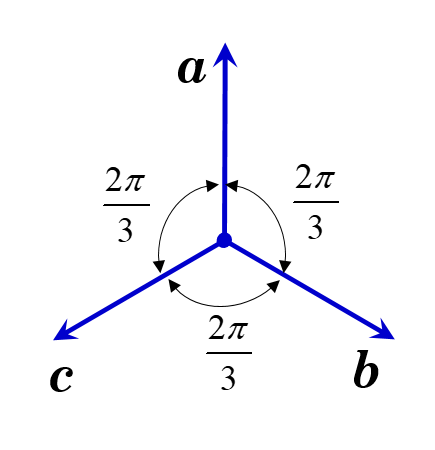
\includegraphics[width=0.3\linewidth]{fig1_2.eps} 
	\end{center}
	\caption{Vectors $\fat{a}, \fat{b}$ and $\fat{c}$ of equal magnitude.} 
	\label{fig:fig1_2}
\end{figure}
\begin{figure}[h]
	\begin{center}
	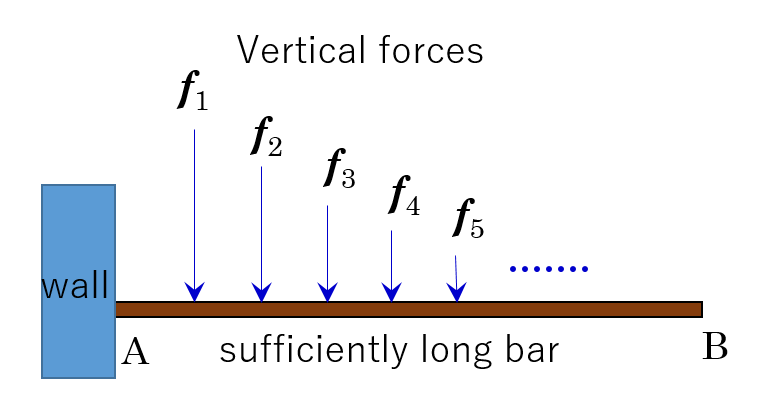
\includegraphics[width=0.5\linewidth]{fig1_3.eps} 
	\end{center}
	\caption{Infinitely many downward forces acting to a horizontally supported bar AB.}
	\label{fig:fig1_3}
\end{figure}
\begin{figure}[h]
	\begin{center}
	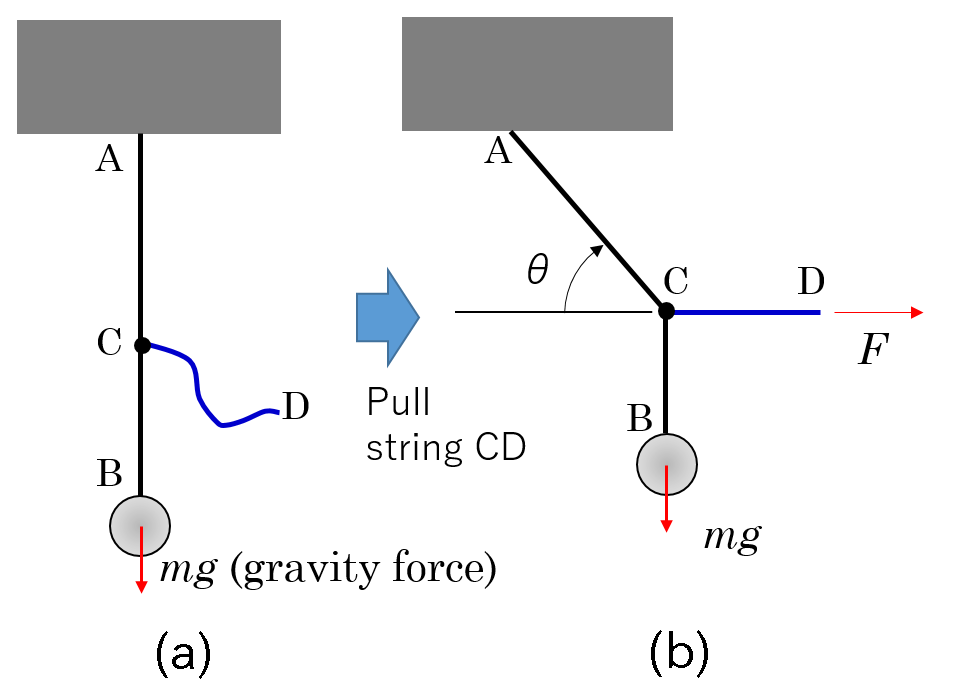
\includegraphics[width=0.6\linewidth]{fig1_4.eps} 
	\end{center}
	\caption{An weight of mass $m$ hung from a ceiling by a string AB.} 
	\label{fig:fig1_4}
\end{figure}
\section*{Problem Set}
\begin{figure}[h]
	\begin{center}
	\includegraphics[width=0.3\linewidth]{fig1_5.eps} 
	\end{center}
	\caption{Vectors $\fat{a}, \fat{b}$ and $\fat{c}$ in 2-dimensional space with an
	xy Cartesian coordinate system.}
	\label{fig:fig1_5}
\end{figure}
\begin{figure}[h]
	\begin{center}
	\includegraphics[width=0.3\linewidth]{fig1_6.eps} 
	\end{center}
	\caption{Vectors $\fat{a}, \fat{b}$ and $\fat{c}$ of equal magnitude.} 
	\label{fig:fig1_6}
\end{figure}
\begin{figure}[h]
	\begin{center}
	\includegraphics[width=0.45\linewidth]{fig1_7.eps} 
	\end{center}
	\caption{Infinitely many vertical forces of alternating direction on 
	a horizontally supported bar AB.}
	\label{fig:fig1_7}
\end{figure}
\begin{figure}[h]
	\begin{center}
	\includegraphics[width=0.45\linewidth]{fig1_8.eps} 
	\end{center}
	\caption{Two weights of different mass hung from a ceiling by strings} 
	\label{fig:fig1_8}
\end{figure}
%%%%%%%%%%%%%%%%%%%%%%%%%%%%%%%%%%%%%%%%%%%%%%%%%%%%%%%%%%%%%%%%
%
% Memo (still to write) 
%  component-wise opreation, multiplication, addition, dot/cross products
%  linearity of cross product
%  Solved and non solved problems
% A guide for on-line study
%  Overview 
%  Objective of class
%  On the subission of reports
\begin{enumerate}
\item
In the first reading, try getting an overall picture of the topics discussed in the class.
You can skim and read casually through the lecture note.
\item
In your second reading, read the lecture note carefully and follow the logical 
	development including definitions, formulas and solved problems.
\item
Close the textbook and try reconstructing what you've learnt.
\item
Solve by yourself the solved problems without looking at the solutions.
\item
Solve the classroom asingment and write up a solution. 
Use A4 paper. Use of a word processor is not necessary as long as your 
handwritten solution is intelgible. 
Scan your answer sheet and submit online via Moodle your PDF scanned solution.
The deadline of submission 
\end{enumerate}
\end{document}
